
Figure~\ref{fig:convergPD} shows the convergence plot for this example, with all parameters converging quickly to their estimated value. 

\begin{figure}[!h]
\begin{center}
\par \kern -1cm
\epsfig{file=figs/PD_convergence.eps,width=11cm,angle=270}
\end{center}
\par \kern -0.5cm
\caption{Convergence plots for the estimated pharmacokinetic parameters and the variabilities.} \label{fig:convergPD}
\end{figure}

Figure~\ref{fig:LLIS} shows the evolution of the log-likelihood during the importance sampling step. Figure~\ref{fig:PDdiagnos} shows the predicted values compared to the observed concentrations, for the population predictions (left) and the individual predictions (right).

\begin{figure}[!h]
\begin{center}
\par \kern -1cm
\epsfig{file=figs/PD_llis.eps,width=9cm,angle=270}
\end{center}
\par \kern -0.5cm
\caption{Estimating the log-likelihood by Importance Sampling.} \label{fig:LLIS}
\end{figure}

\begin{figure}[!h]
\begin{center}
\par \kern -1cm
\epsfig{file=figs/PD_diagnos.eps,width=11cm,angle=270}
\end{center}
\par \kern -0.5cm
\caption{Basic diagnostic plots.} \label{fig:PDdiagnos}
\end{figure}

%%%%%%%%%%%%%%%%%%%%%%%%%%%%%%%%%%%%
We can run 
In this example, the likelihood obtained by importance sampling is somewhat different from the likelihood obtained by linearisation of the model. We first increased the number of MCMC samples to check that the likelihood by importance sampling was indeed stable.
\par \kern -0.3cm
\begin{verbatim}
saemix.fit["options"]$nmc.is<-10000
saemix.fit<-llis.saemix(saemix.fit)
\end{verbatim}

\par \kern -0.2cm
The results, shown in figure~\ref{fig:cow.LLIS}, indicate that the estimate obtained with 5000 MCMC samples (the default number), is probably sufficient.
\begin{figure}[!h]
\begin{center}
\par \kern -0.5cm
\epsfig{file=figs/cow_llis.eps,width=9cm,angle=270}
\end{center}
\par \kern -0.5cm
\caption{Estimating the log-likelihood by Importance Sampling for the {\sf cow} dataset.} \label{fig:cow.LLIS}
\end{figure}

\clearpage
\newpage
